% Chapter 4

\chapter{Architecture}

\begin{figure}[htbp]
    \centering
%    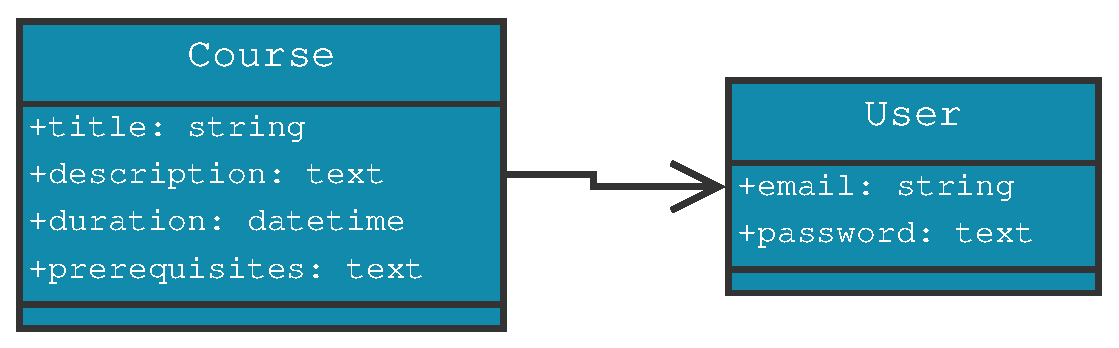
\includegraphics{discite}
    \rule{35em}{0.5pt}
    \caption[Class Diagram]{Class Diagram in UML}
    \label{fig:Class Diagram}
\end{figure}

% let's define some commands to include the test suite
\newcommand{\lTest[1]}{\lstinputlisting[style=ruby]{/home/dimon/sandbox/rails/discite/spec/\string#1}}
\newcommand{\lFeatureTest[1]}{\lstinputlisting[style=ruby]{/home/dimon/sandbox/rails/discite/spec/features/\string#1}}
\newcommand{\lPagesTest[1]}{\lstinputlisting[style=ruby]{/home/dimon/sandbox/rails/discite/spec/pages/\string#1}}

\lTest[spec_helper.rb]
\lFeatureTest[home_spec.rb]
\lPagesTest[home_page.rb]

This thesis has described the design and the implementation of a peer-to-peer
teaching network.\\
\# to add
\begin{itemize}
\item overall description of the resulted system
\item what choices where good and what bad
\item what could we have chosen that would have had better results
\item statistics of visitors, maybe testimonials of early users?
\end{itemize}
\section{Possible Improvements}
Implementation of a management dashboard for the teacher, to allow better course
management. The software is does not currently provide means to block abusive
the students. Also there is no form of selecting the student. A enrollment key
system can be implemented.
